\chapter{Evaluation}

This section is focused on the empirical evaluation of \textsc{Carico} as a Kubernetes
scheduler. As I was unable to find any telemetric-only schedulers, I decided to
compare \textsc{Carico} against the default Kubernetes scheduler throughout this section.
\texttt{kube-scheduler} is an industry-standard scheduler that was built upon
the lessons learnt from Borg \cite{}, and thus, has been thoroughly optimised
and battle tested. As \texttt{kube-scheduler} is a Pod description-based
scheduler, I use mutliple different resource requests to highlight how the
performance achieved can vary depending on description.

The chapter is divided into the following sections:
\textbf{Overhead - Section \ref{sec:eval-overhead}:} I measure the computational overhead
incurred from running the \textsc{Carico} Pods on every Node. To ascertain this effect, I
complare the Job Completion time with and without the deployment of the \textsc{Carico}
Pod DaemonSet

\textbf{Different Workloads - Sections
\ref{sec:eval-cpu-centric},\ref{sec:eval-mem-centric}, \ref{sec:eval-mixed}:}
These sections investigate the performance of \textsc{Carico} when deploying different
workloads. For each workload, I investigate four metrics: Job Completion, Number
of Running Pods, Pod Completion and Resource Usage. Job Completion measures the
time it takes for all the Pods specified by a Job to complete. This then acts as
a strong indicator of overall throughput of a scheduler. The Number of Running
Pods will be used to explain the achieved Job Completion. Pod Completion instead
focuses on the distribution of the time it takes for the Pods to complete. The
distribution gives an indication of the amount of contention that occurs during
the deployment of the Job. A tail-heavy distribution indicates high levels of
contention and that the scheduler is overloading a Node. Finally, resource
utilisation will focus on CPU and Memory utilisation. I decided to only measure
these two resources as they are the only two that are currently considered in
the scheduling decisions made by both \textsc{Carico} and the default Kubernetes
scheduler.

\textbf{Workload Isolation - Section \ref{sec:workload-isolation}:} In this
section I investigate the workload-isolation provided by \textsc{Carico} and the default
Kubernetes scheduler. Workload isoolation is considered a core component of QoS
scheduling, and thus is a useful metric to observe.

\section{Evaluation Setup}
These experiments ran on a Kubernetes cluster containing 20 virtual machines
(VMs) running on the Xen hypervisor. One of the machines is used as the master
Node, and the rest are worker Nodes. The master Node contains all the Pods in
the control plane, and during the evaluation of \textsc{Carico}, it contains the \textsc{Carico}
Scheduler and Aggregation Server. Each VM features four Intel Xeon Gold 6142
CPUs \@ 2.60Ghz with 8 GB of RAM running Ubuntu 24.04.2 LTS. Each CPU has a
single core with hyperthreading disabled. When running \texttt{kubectl describe
nodes}, each Node advertises $4000$ milli-CPU seconds and 8GB of RAM.

During the evaluation, I use a Prometheus deployment \cite{} to collect various
statistics, such as running Pod count, resource utilisation and Kubernetes
object completions.

\section{\textsc{Carico} Overhead}
\label{sec:eval-overhead}
To measure the overhead incurred from running the \textsc{Carico} pods on the Nodes, I
compared the completion time of Jobs when running on Nodes with and without the
\textsc{Carico} deployment. I considered easuring resource utilisation on a Node with
just the \textsc{Carico} Pod running, but much of the behaviour of the
\textsc{Carico} Pod occurs during container events. As a result, the measured overhead
would not represent the entire impact of the \textsc{Carico} Pod. Instead, by measuring
the overhead over Jobs, we aggregate the impact of \textsc{Carico} across multiple
container events, providing a more holistic view of its impact.

\begin{table}[ht!]
\centering
    \begin{tabular}{|c|c|}
    \hline
    \textbf{Number of Pods} & \textbf{\% Overhead with \textsc{Carico}} \\
    \hline
        100 & -2.33 $\pm$ 3.29 \\
        250 & -1.19 $\pm$ 2.44 \\
        500 & 4.84  $\pm$ 1.25 \\
        750 & 1.69  $\pm$ 0.42 \\
        1000 & 2.27  $\pm$ 0.66 \\
    \hline
    \end{tabular}
    \label{tab:overhead}
    \caption{The overhead incurred when running \textsc{Carico} Pods on Nodes during the
    executing of Jobs with varying Pod counts. Each Pod executed
    \texttt{bpi(2000)} and requested 200 milliseconds of CPU time.}
\end{table}

To measure \textsc{Carico}'s overhead, I used Pod's executing \texttt{bpi(2000)}. Table
\ref{tab:overhead} presents the relative change in Job Completion time with
\textsc{Carico} Pods running on the Nodes. We can see that the Job Completion time of
smaller Jobs are more noisy, therefore, resulting in an observed decrease in Job
Completion times. However, with larger and more stable Jobs, the overhead from
\textsc{Carico} is more visible. From these observations we can conclude that \textsc{Carico} has
$\approx$ 2\% overhead.
%
% For any practical projects, you should almost certainly have some kind
% of evaluation, and it's often useful to separate this out into its own
% chapter.
\section{CPU-centric Workloads}
\label{sec:eval-cpu-centric}
For this experiment, I used a CPU-heavy workload: Pods calculatig $\pi$ to 2000
digits (\texttt{bpi(2000)}). This simple workload helps visualise the impact of
combining CPU Pressure with CPU Utilisation.

\subsection{Throughput}
During the measurements with the default Kubernetes scheduler, I used the
following CPU requests: 100m, 200m, 500m, 1000m. The results are given in Table
\ref{tab:pi-2000-throughput}

\begin{table}[ht!]
\centering
    \begin{tabular}{|l|r|c|c|c|c|c|}
    \hline
    \textbf{Scheduler} & \textbf{Requested} & \multicolumn{5}{c|}{\textbf{Job Completion (s)}} \\
    \cline{2-7}
    &  \textbf{CPU} & \textbf{100 Pods} & \textbf{250 Pods} & \textbf{500 Pods} & \textbf{750 Pods} & \textbf{1000 Pods} \\
    \hline
    Default & 100m & 15.7 $\pm$ 0.6 & 31.7 $\pm$ 2.1 & 56 $\pm$ 1.7 & 84.7 $\pm$
        0.6 & 112 $\pm$ 0.0 \\
    Default & 200m & 15.7 $\pm$ 0.7 & 30.7 $\pm$ 0.6 & 55 $\pm$ 1 & 79 $\pm$ 0.0
        & 103 $\pm$ 1 \\
    Default & 500m & 15.7 $\pm$ 1.2 & 32 $\pm$ 2.6 & 57.7 $\pm$ 0.6 & 81 $\pm$ 2
        & 104 $\pm$ 2.1 \\
    Default & 1000m & 21 $\pm$ 2.0 & 54.7 $\pm$ 0.6 & 96 $\pm$ 2.6 & 133 $\pm$
        0.6 & 175 $\pm$ 1 \\
    \textsc{Carico} &  & 20.3 $\pm$ 0.6 & 35.3 $\pm$ 0.6 & 60.3 $\pm$ 2.5 & 89 $\pm$ 2 &
        109$\pm$ 1 \\
    \hline
    \end{tabular}
    \caption{Job Completion of Job deployments with different Pod counts. Each
    Pod executed \texttt{bpi(2000)}. For the default scheduler, the requested
    resources are also given}
    \label{tab:pi-2000-throughput}
\end{table}

From Table \ref{tab:pi-2000-throughput}, we can see how much the performance of
the default scheduler varies depending on the amount of CPU time requested.
Over-estimating requests can result in the CPU being underutilised, while
under-estimating can result in too many Pods running on a Node at once. With
\textsc{Carico}, we observed only observed a 10\% reduction in Job Completion time. This
can be attributed to its use of telemetric data: CPU utilisation amd CPU
Pressure. In Section \ref{sec:issue-with-util}, I investigated these metrics and
showed how with \texttt{bpi(2000)} Pods, these metrics indicated full capacity
when running 4-8 Pods. As the capacity signal of a Node is tied to these
metrics, the Node's will never advertise more capacity than $\approx$ 8 Pods.

TODO: POTENTIALLY MENTION HOW 1000M AND 500M CORRESPOND TO THE LIMIT OF USING
CPU UTILISATION AND CPU PRESSURE

\subsection{Pod Completions}
\begin{table}[ht!]
\centering
    \begin{tabular}{|l|r|c|c|c|c|c|c|c|}
    \hline
        \bfseries Scheduler & \bfseries CPU Request & \bfseries Mean & \bfseries Std. &
        \bfseries Min. & \bfseries 25\% & \bfseries Median & \bfseries 75\% & \bfseries Max. \\
    \hline
        Default & 100m & 47.43 & 14.59 & 7.00 & 39.00 & 52.00 & 57.00 & 73.00
        \\
        Default & 500m & 9.55 & 1.49 & 5.00 & 9.00 & 10.00 & 10.00 & 14.00
        \\
        \textsc{Carico} & & 7.69 & 0.99 & 5.00 & 7.00 & 8.00 & 8.00 & 11.00 \\
    \hline
    \end{tabular}
    \caption{Pod Completion of multi-resource Job deployments with different Pod
    counts. For the default scheduler, \texttt{bpi(2000)} Pods requested 100
    milliseconds of CPU and ML Pods requested 200 milliseconds CPU and 750Mi of
    memory}
    \label{tab:cpu-pod-completions}
\end{table}
I decided to further investigate the behaviour of the schedulers by measuring
the Pod Completion time given in Figure \ref{tab:cpu-pod-completions}. From this
table, we observe that the lower request default schedulers ends up with a very
tail-heavy distribution for Pod Completions. Increasing the request to 500
milliseconds, reduces the mean by $\approx$ 80\% while also reducing the skew.
However, \textsc{Carico} is able to achieve the lowest Pod Completion distribution. To
help explain the reason by this result, I also measured the number of Pods
running on each Nodes during the Job execution, and present the values in Figure
\ref{fig:pi-2000-1000x-pod-running}.

\begin{figure}[ht!]
    \centering
    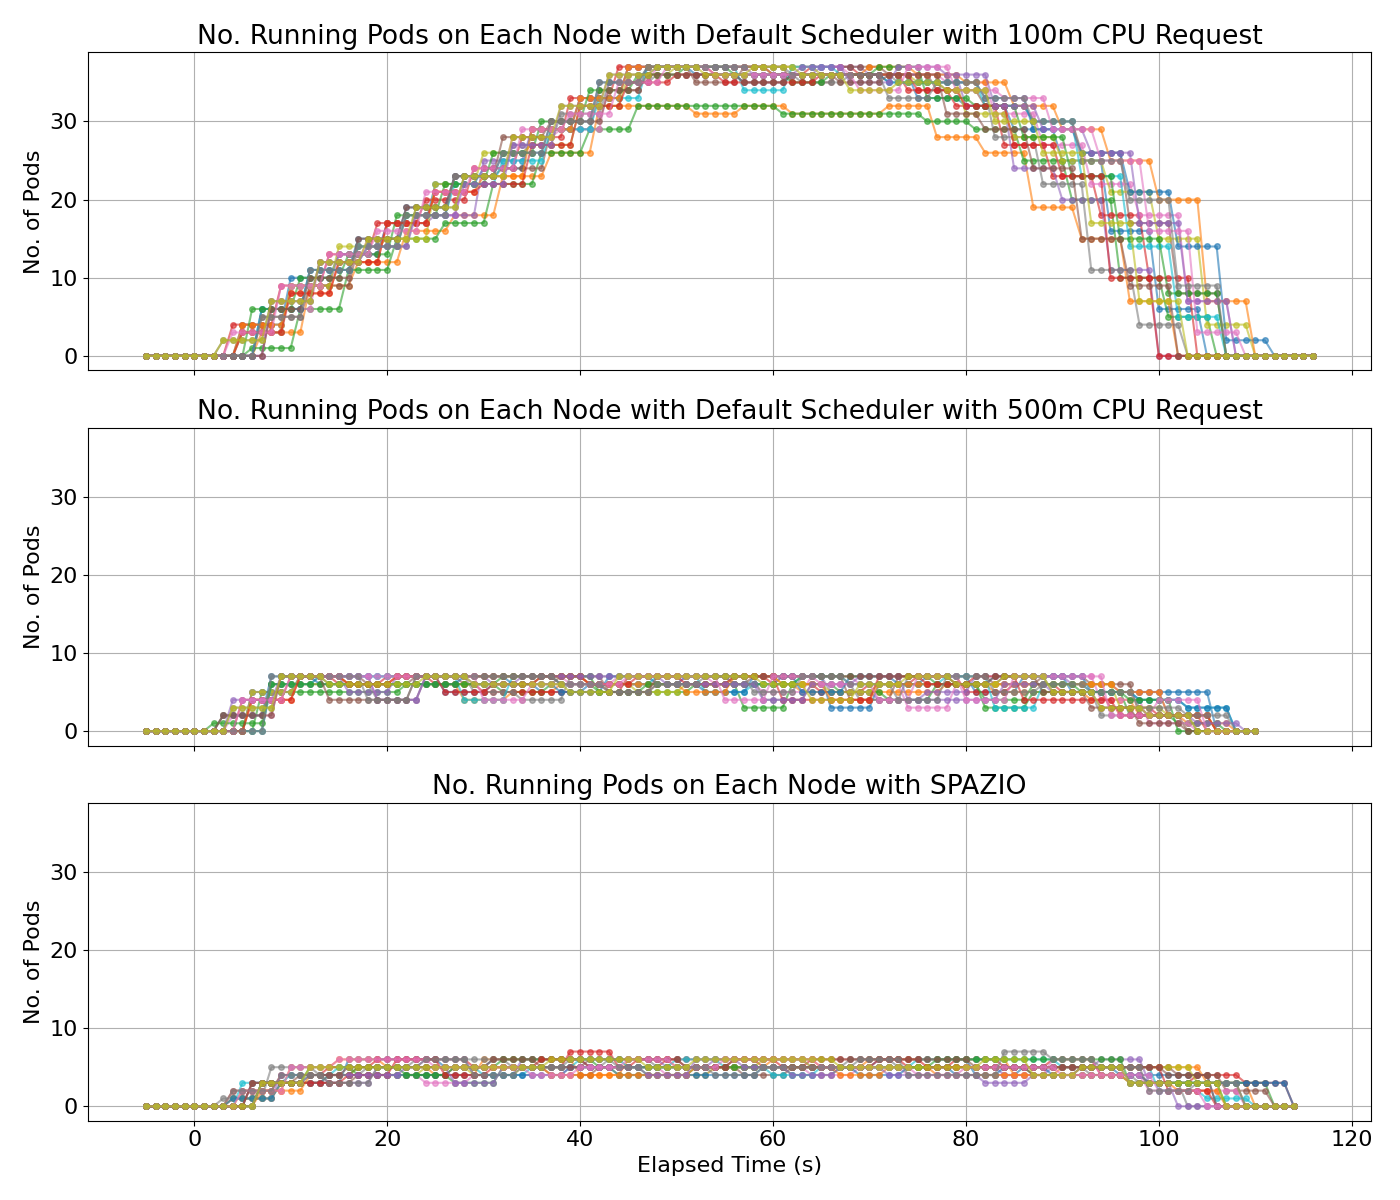
\includegraphics[width=\textwidth]{images/pi-running-pods.png}
    \caption{The number of \texttt{bpi(2000)} Pods running on a Node during the
    execution of a Job with 1000 Pods.}
    \label{fig:pi-2000-1000x-pod-running}
\end{figure}
Figure \ref{fig:pi-2000-1000x-pod-running} depicts the different approaches
taken by each scheduler. As the default Kubernetes Scheduler tackles scheduling
as if it were a bin-packing problem, it schedules as many pods that can fit on a
Node; each Node has 4000m CPU capacity, 1000m per core. As a result, the 100m
request results in a stampede of Pods while the 500m request and \textsc{Carico} assign
a relatively constant number of Pods. However, the default scheduler with 500m
Pods takes the edge in terms of throughput as it achieves a higher number of
running Pods per Node.


TODO: SHOULD I TALK ABOUT NOT OVERPROVISIONING AS MEMORY USES OOM KILLS IF FULL
AND THEREFORE RISKED CORRECTNESS OF SIGNAL

\subsection{Resource Utilisation}
\begin{figure}[h]
    \centering
    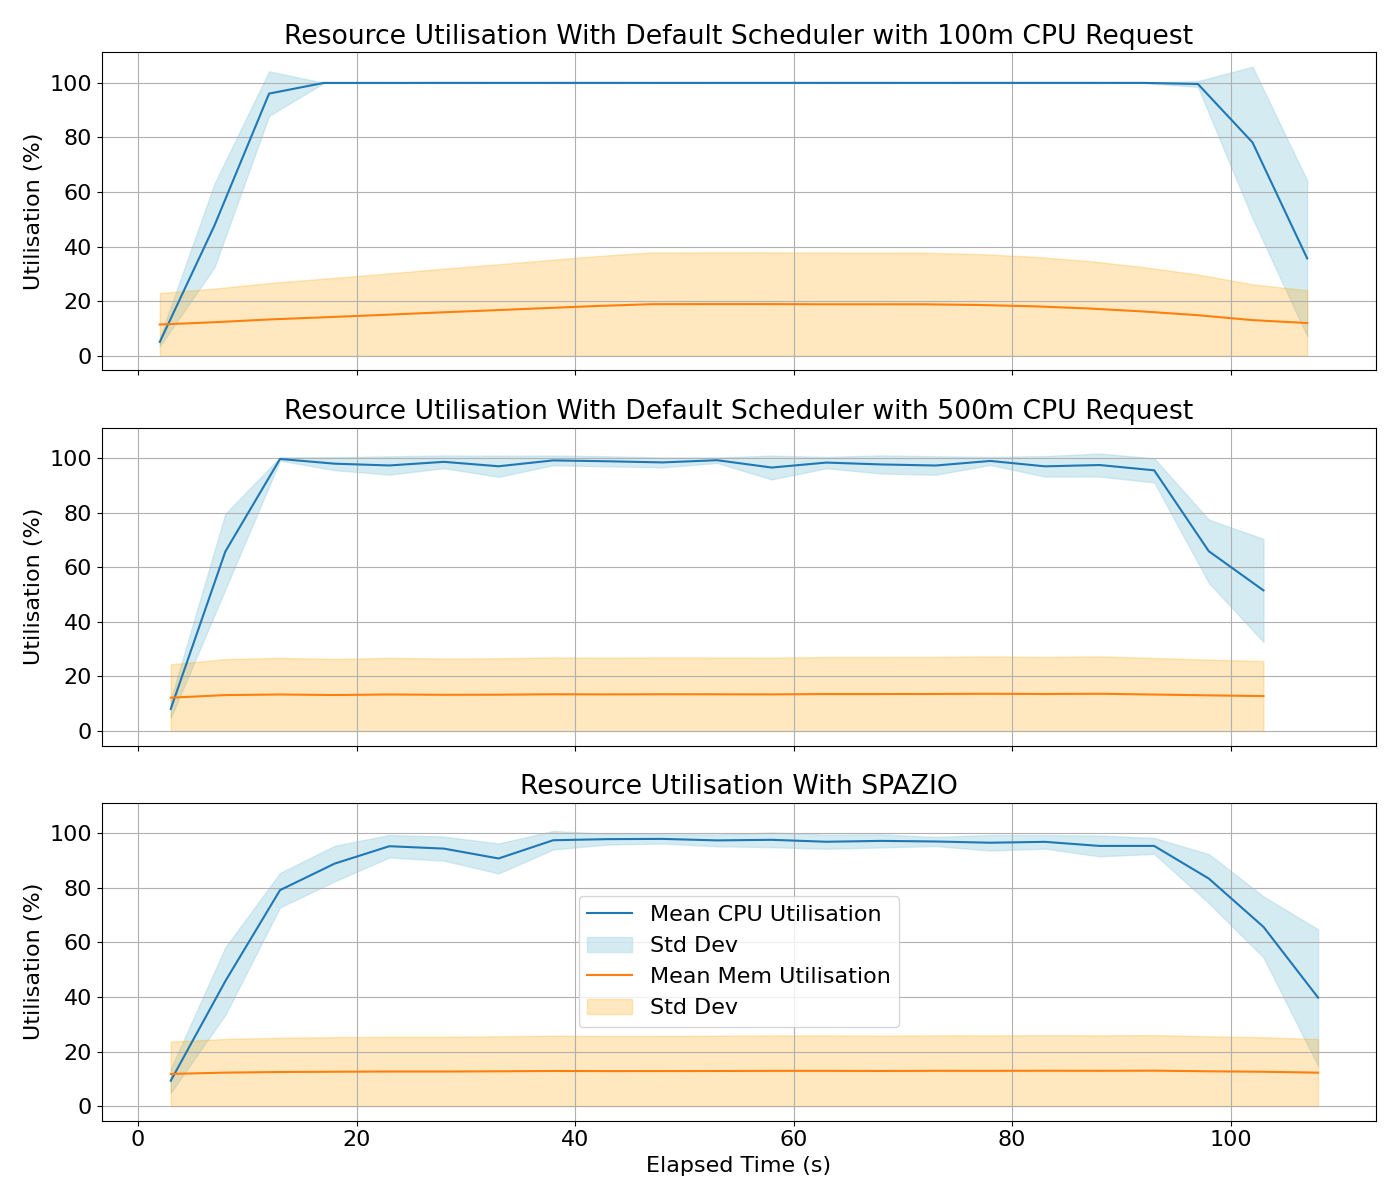
\includegraphics[width=\textwidth]{images/pi-util.png}
    \caption{the resource utilisation when scheduling a job with 1000 pods
    executing \texttt{bpi(2000)}. the top figure gives the resource utilisation
    when scheduling with the default kubernetes scheduler. The bottom figure
    gives the resource utilisation when scheduling with spazio.}
    \label{fig:pi-2000-1000x-pod-util}
\end{figure}

Figure \ref{fig:pi-2000-1000x-pod-util} shows the resource utilisation during
the execution of a Job with 1000 Pods. The default Kubernetes scheduler with
100m CPU requests achieves 100\% CPU utilisation due to the large number of Pods
running on each Node. The resulting allocation even results in a visible
increase in the Memory usage.

\section{Memory-centric Workloads}
\label{sec:eval-mem-centric}
In this experiment, I use a Job that specifies Pods that performed a small ML
workload. This workload uses a significant amount of memory, which unlike CPU,
must be carefully handled. If we increase the number of processes on a
fully-utilised CPU, it only results in each process having a smaller portion of
CPU time and degrading its performance. On the other hand, memory is less
forgiving as once memory runs out, the kernel begins OOM killing processes. This
be detrimental to Job Completion, as terminated Pods results in wasted
computations.

\subsection{Throughput}
\begin{table}[ht!]
\centering
    \begin{tabular}{|l|r|r|c|c|}
    \hline
    \textbf{Scheduler} & \multicolumn{2}{c|}{\textbf{Requested}} &
        \multicolumn{2}{c|}{\textbf{Job Completion (s)}} \\ \cline{2-5}
    &  \textbf{CPU} & \textbf{Memory} & \textbf{100 Pods} & \textbf{200 Pods} \\
    \hline
        Default & 200m & 750Mi & 144.3 $\pm$ 0.6 & 362 $\pm$ 20.4\\
        \textsc{Carico} &  &  & 189 $\pm$ 4.36 & 353.3 $\pm$ 12.7 \\
    \hline
    \end{tabular}
    \caption{Job Completion of Job deployments with different Pod counts. Each
    Pod executed a small ML workload. For the default scheduler, the requested
    resources are also given}
    \label{tab:ml-throughput}
\end{table}
The Job Completions from the experiment are given in Table
\ref{tab:ml-throughput}. \textsc{Carico} achieves a worse performance in the smaller 100
Pod Job, but actually overtakes the default Kubernetes scheduler with the 200
Pod Job.

\subsection{Pod Completions}
\begin{table}[ht!]
\centering
    \begin{tabular}{|l|r|c|c|c|c|c|c|c|}
    \hline
        \bfseries Scheduler & \bfseries \# Pods & \bfseries Mean & \bfseries Std. &
        \bfseries Min. & \bfseries 25\% & \bfseries Median & \bfseries 75\% & \bfseries Max. \\
    \hline
        Default & 100 & 127.38 & 5.29 & 118 & 123.00 & 126.00 & 132.00 &
        138.00 \\
        \textsc{Carico} & 100 & 59.02 & 14.62 & 27.00 & 55.00 & 61.00 & 66.00 & 94.00 \\
        Default & 200 & 225.19 & 36.19 & 45.00 & 231.00 & 236.00 & 239.00 &
        244.00\\
        \textsc{Carico} & 200 & 64.46 & 14.33 & 23.00 & 57.75 & 67.00 & 73.25 & 89.00 \\
    \hline
    \end{tabular}
    \caption{Pod Completion of multi-resource Job deployments with different Pod
    counts. For the default scheduler, \texttt{bpi(2000)} Pods requested 100
    milliseconds of CPU and ML Pods requested 200 milliseconds CPU and 750Mi of
    memory}
    \label{tab:mem-pod-completions}
\end{table}

Table \ref{tab:mem-pod-completions} gives the Pod Completion Distribution of the
ML-based Jobs. When using the default Kubernetes scheduler, increasing the Pod
count in a Job where the resource request is underestimated, increases
drastically the average Pod Completion time as well as skewing the distribution
to become more tail-heavy. However, the distribution of Pod Completion Time
achieved by \textsc{Carico} remains consistent as you increase the Job size.

\begin{figure}[ht!]
    \centering
    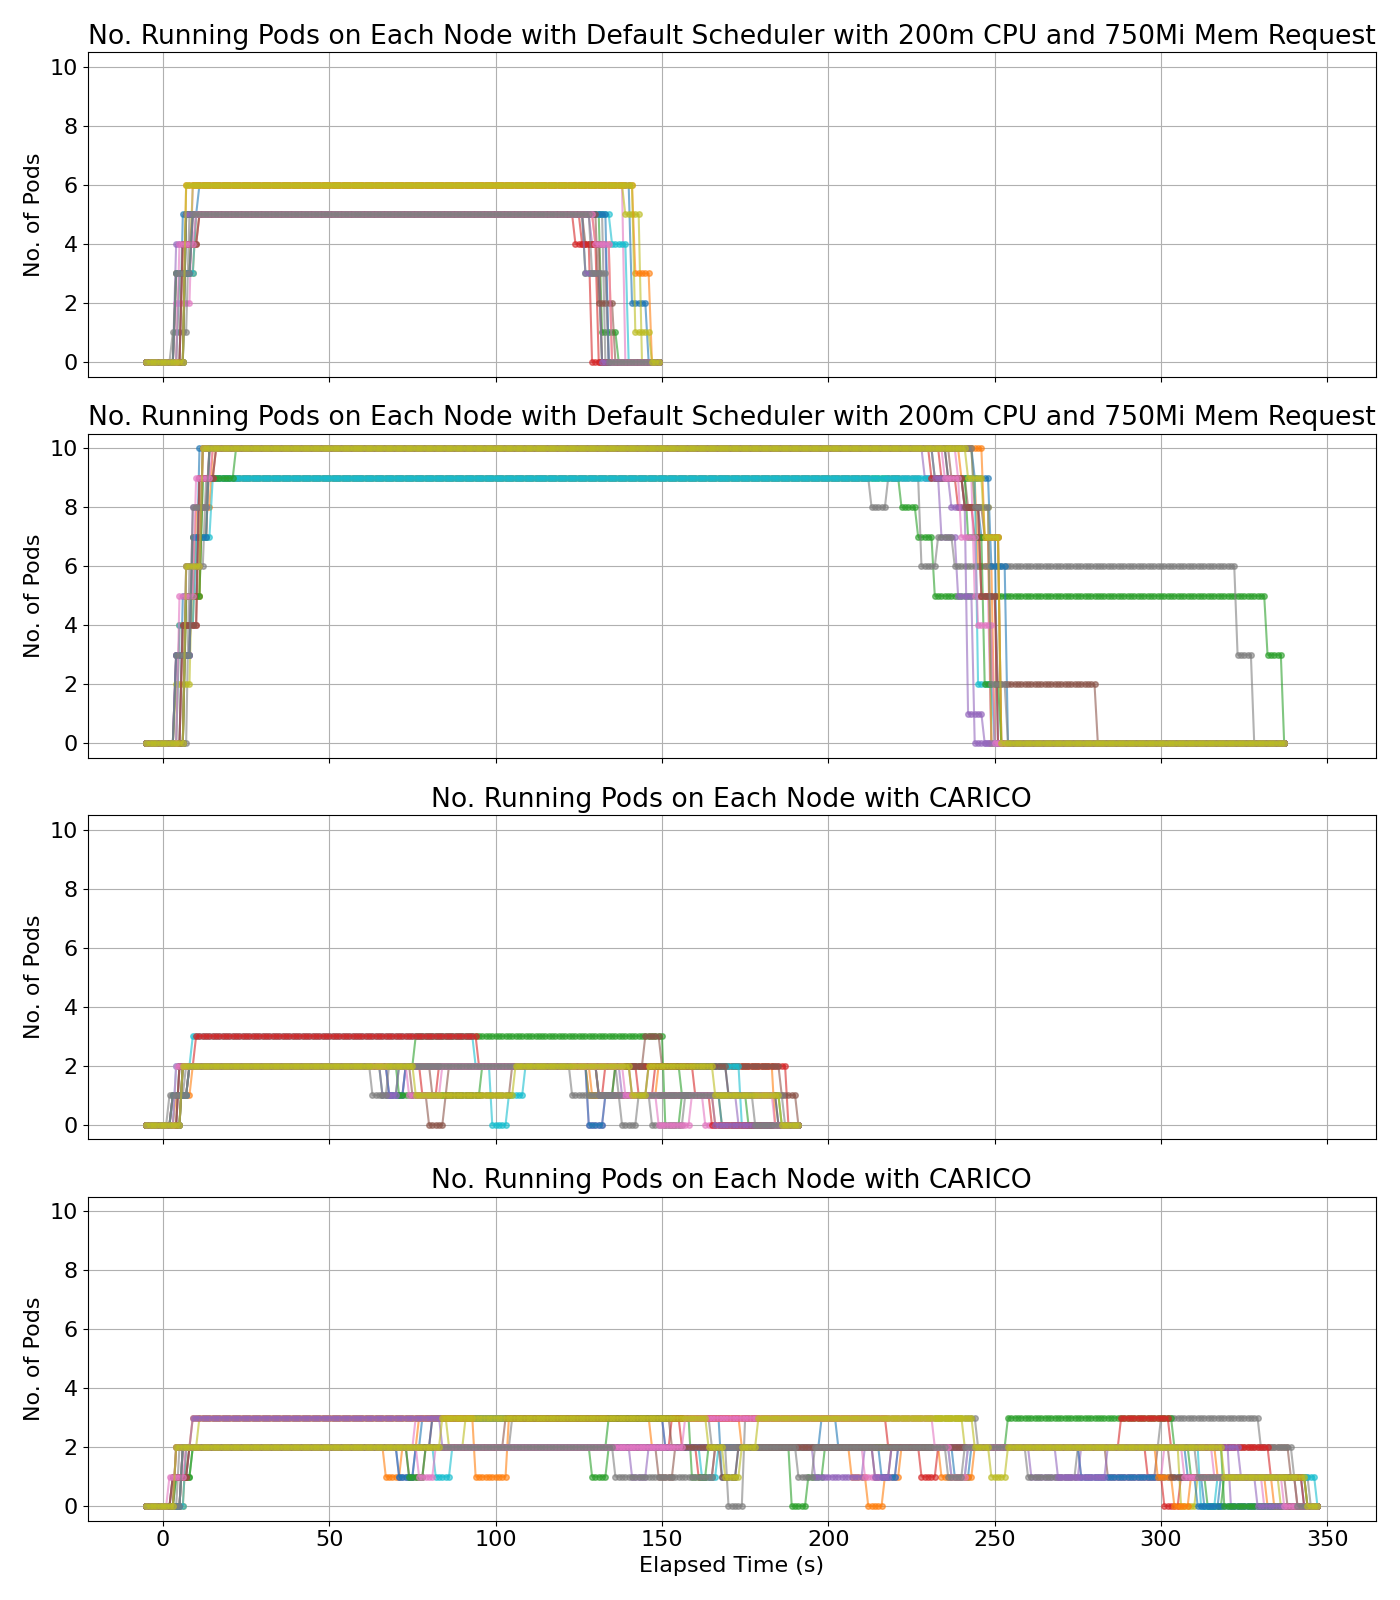
\includegraphics[width=\textwidth]{images/ml-running-pods.png}
    \caption{The number of ML Pods running on a Node during the
    execution of a Job with 100 and 200 Pods.}
    \label{fig:ml-pod-running}
\end{figure}
Figure \ref{fig:ml-pod-running} depicts the number of Pods running on each Node
at a given time. We can see how in the larger ML Job, the default scheduler is
able to allocate a majority of the Pods across the Nodes. Each Node advertises
$\approx$ 8GB of memory while each Pod requests 750MiB of Memory. All these Pods
end up competing for resources, and the overcontention increases individual
Pod completion time. The scheduler still has to wait for Pods to terminate to
free up memory. When space does become available, it is because a
stampede of Pods have terminated. While, the scheduler was able to now allocate
the remaining Pods, only a few Nodes are used while the rest become idle. This
second wave of Pods results in a slower throughput compared \textsc{Carico} which ensures
1-3 Pods are always running on a Node.

\subsection{Resource Utilisation}
\begin{figure}[ht!]
    \centering
    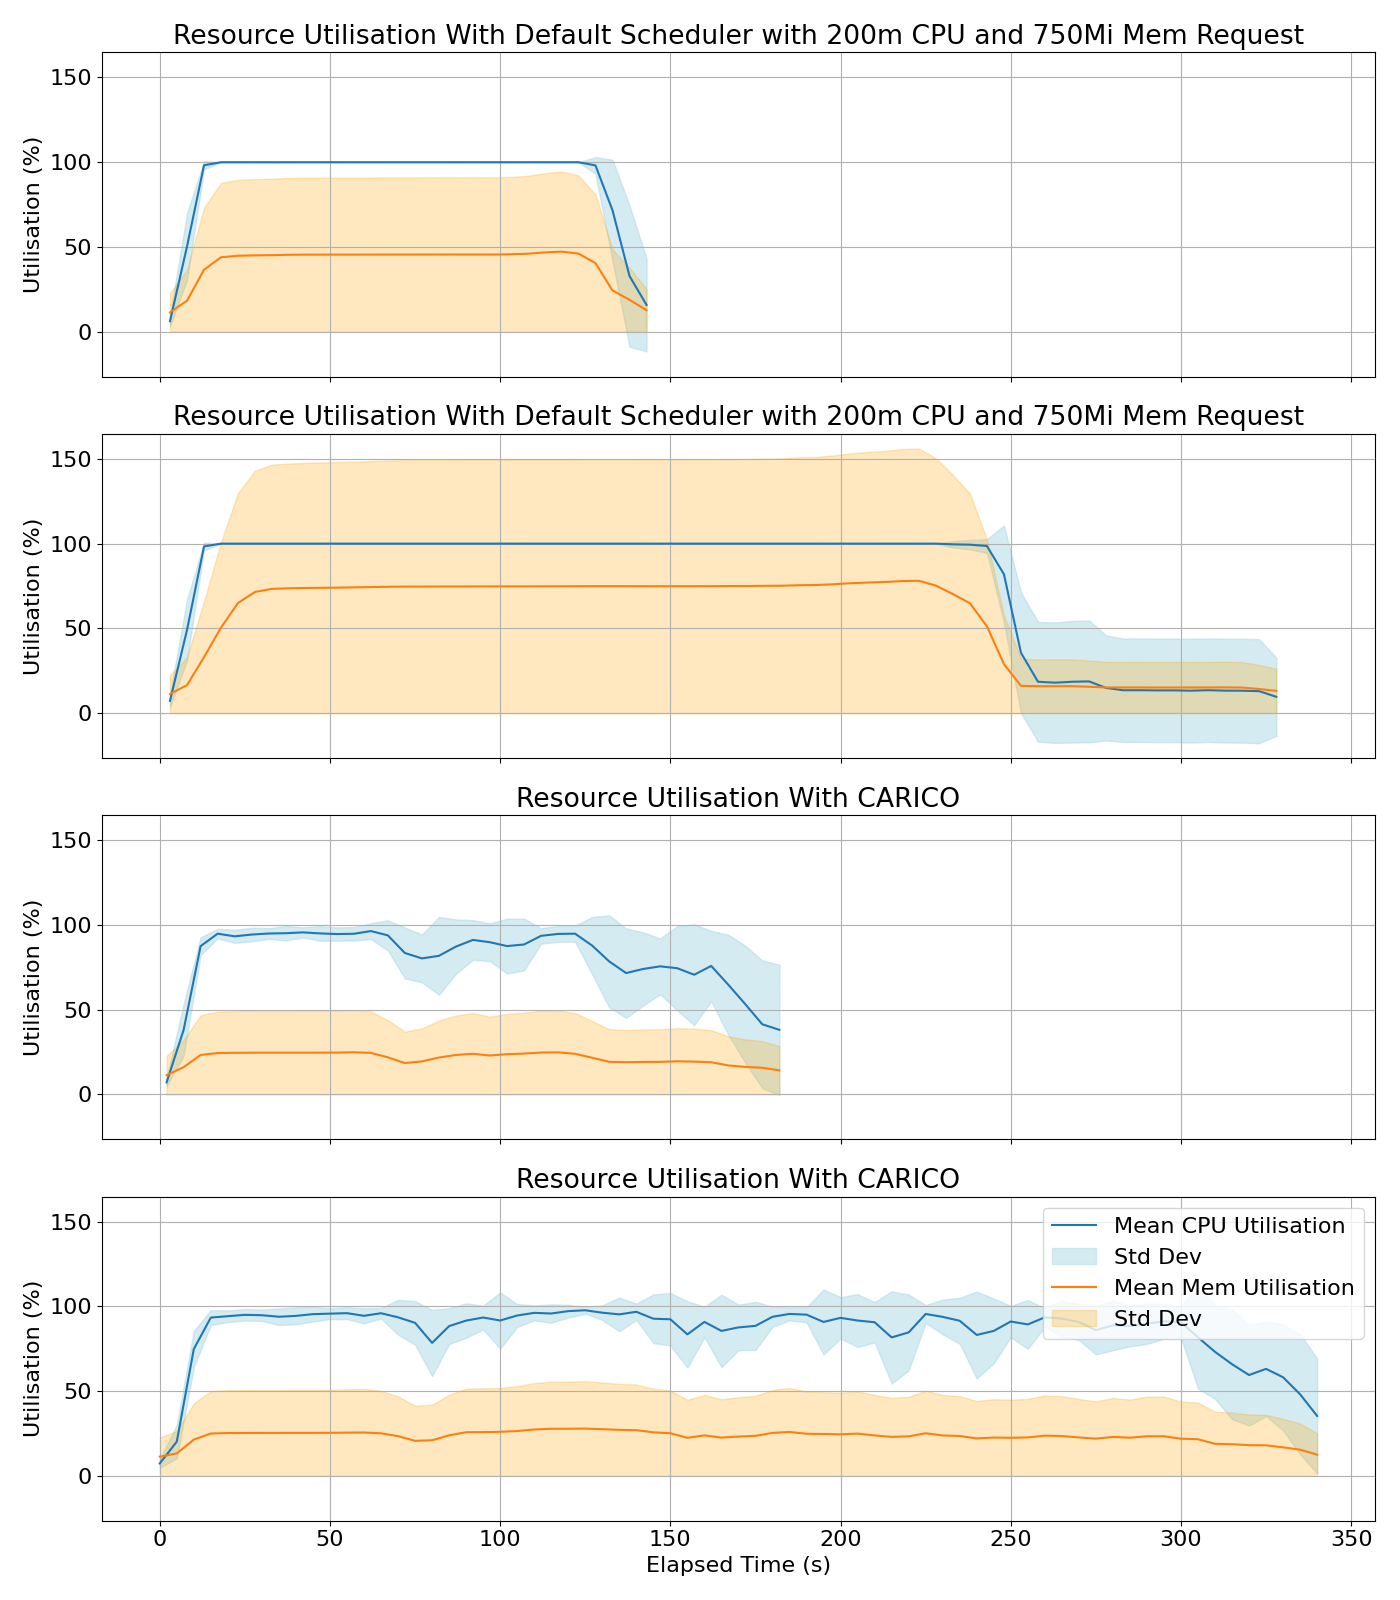
\includegraphics[width=\textwidth]{images/ml-util.png}
    \caption{The resource utilisation when scheduling a Job with 1000 Pods
    executing \texttt{bpi(2000)}. The top figure gives the resource utilisation
    when scheduling with the default Kubernetes scheduler. The bottom figure
    gives the resource utilisation when scheduling with \textsc{Carico}.}
    \label{fig:ml-util}
\end{figure}

Figure \ref{fig:ml-pod-running} also helps to explain the resulting resource usage
depicted in Figure \ref{fig:ml-util}. While the ML workload is memory-intense,
it still contributes significantly to CPU utilisation. As the default scheduler
does not actively look at resource utilisation, it is able to allocate Pods to
Node's with fully-utilised CPUs. As a result, it achieves a higher memory usage
with both Jobs. However, we can also observe the effect of the second wave of
Pod allocations during the 200 Pod Job. During the last minute of the Job's
executing, the average CPU and Memory utilisation of the cluster have dropped to
$\approx$ 10\%; barely above their baseline utilisation.
On the other hand, \textsc{Carico} is again limited by the Node's CPU metrics, achieving
a lower overall memory utilisation.

\section{Mixed Workloads}
\label{sec:eval-mixed}
In this experiment, I deployed the two Jobs defined above: a short-lived
CPU-focused workload and a longer running ML workload. This experiment evaluates
how \textsc{Carico} handles more than one type of workload.

\subsection{Throughput}
To thoroughly evaluate \textsc{Carico} in this scenario, I varied the distribution of
Pods from each Job. The observed Job Completions are given in Table
\ref{tab:mixed-throughput}.

\begin{table}[ht!]
\centering
    \begin{tabular}{|l|c|c|c|}
    \hline
    \textbf{Scheduler} & \multicolumn{2}{c|}{\textbf{Job Size}} &
        \textbf{Job Completion (s)} \\ \cline{2-3}
        &  \texttt{bpi(2000)} & \texttt{ML} & \\
    \hline
        Default & 500 & 20 & 105.7 $\pm$ 10.6 \\
        \textsc{Carico} & 500 & 20 & 88.7 $\pm$ 2.5 \\
        Default & 250 & 50 & 118 $\pm$ 4.58 \\
        \textsc{Carico} & 250 & 50 & 115.7 $\pm$ 0.58 \\
        Default & 100 & 100 & 149 $\pm$ 0.0 \\
        \textsc{Carico} & 100 & 100 & 192 $\pm$ 4.0 \\
    \hline
    \end{tabular}
    \caption{Job Completion of multi-resource Job deployments with different Pod
    counts. For the default scheduler, \texttt{bpi(2000)} Pods requested 100
    milliseconds of CPU and ML Pods requested 200 milliseconds CPU and 750Mi of
    memory}
    \label{tab:mixed-throughput}
\end{table}
The Job Completions from the experiment are given in Table
\ref{tab:mixed-throughput}. \textsc{Carico} achieves a higher throughput during the
500-20 and 250-50 combined workloads. However, the final 100-100, we see how the
limiting throughput is now governed by the throughput achieved with the
memory-centric workload.

\subsection{Pod Completions}
Due to \textsc{Carico}'s lackluster throughput, I decided to investigate distribution of
Pods across Nodes and how it impacted Pod Completion times.

\begin{table}[ht!]
\centering
    \begin{tabular}{|l|c|c|c|c|c|c|c|c|}
    \hline
        \bfseries Scheduler & \bfseries Job & \bfseries Mean & \bfseries Std. &
        \bfseries Min. & \bfseries 25\% & \bfseries Median & \bfseries 75\% & \bfseries Max. \\
    \hline
        Default & \texttt{pi-2000} & 28.78 & 7.52 & 7.00 & 27.00 & 30.00 & 33.00 & 45.00 \\
        Default & ML & 65.25 & 10.53 & 49.00 & 58.25 & 64.00 & 75.25 & 82.00 \\
        \textsc{Carico} & \texttt{pi-2000} & 7.40 & 1.14 & 5.00 & 7.00 & 7.00 & 8.00 & 11.0 \\
        \textsc{Carico} & ML & 34.50 & 7.39 & 22.00 & 27.50 & 36.00 & 40.25 & 44.00 \\
    \hline
    \end{tabular}
    \caption{Pod Completion of multi-resource Job deployments with different Pod
    counts. For the default scheduler, \texttt{bpi(2000)} Pods requested 100
    milliseconds of CPU and ML Pods requested 200 milliseconds CPU and 750Mi of
    memory}
    \label{tab:mixed-pod-completions}
\end{table}

Table \ref{tab:mixed-pod-completions} gives the Pod Completion Distribution
during an execution of the 500-20 Job combination. We can observe that the
Pod Completion times for both Jobs is significantly higher with the default
scheduler compared to \textsc{Carico}. This shows how \textsc{Carico} is still able to achieve a
low-tailed Pod Completion time when scheduling workloads with different resource
requests.

% TODO: SHOULD I ONLY INVESTIGATE WORKLOADS WE HAVE SEEN BEFORE SO THAT I CAN
% COMPARE THE CHANGE IN DISTRIBUTION

\begin{figure}[ht!]
    \centering
    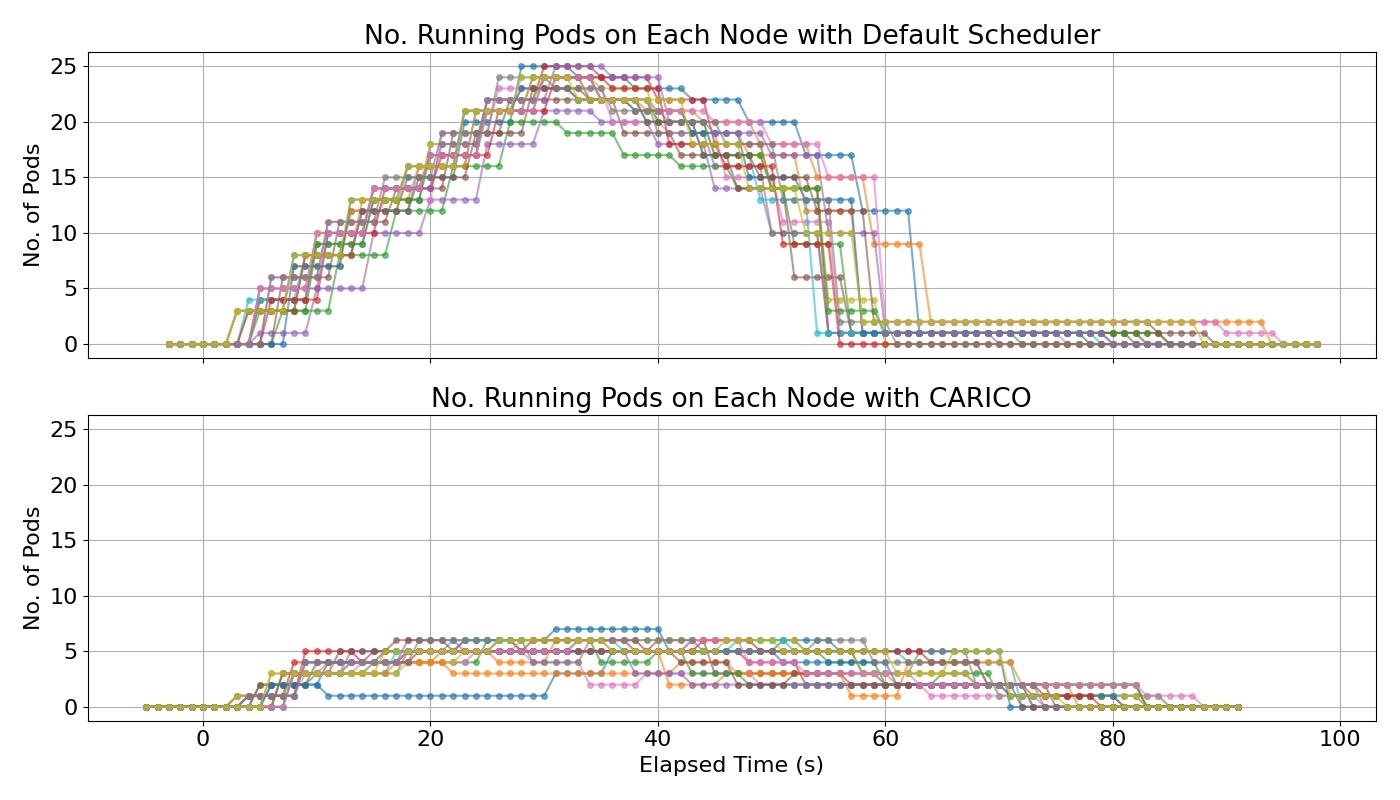
\includegraphics[width=\textwidth]{images/mixed-running-pods.png}
    \caption{The number of Pods running on a Node during the
    500-20 Job combination.}
    \label{fig:mixed-pod-running}
\end{figure}

Figure \ref{fig:mixed-pod-running} depicts the number of Pods running on each Node
at a given time. Like in \ref{fig:ml-pod-running}, the default scheduler ends up
with long-running Pods on small percentage of the Nodes in the cluster. The
default scheduler see that the Node's have enough advertised capacity, and
therefore, allocate all the Pods as they arrive. This again results in a
stampede of completions, and only a few Nodes continue to do work. However,
\textsc{Carico}'s rate of Pod allocation remains consistent, ensuring that Nodes have a
close to constant number of Pods.

\subsection{Resource Utilisation}

\begin{figure}[ht!]
    \centering
    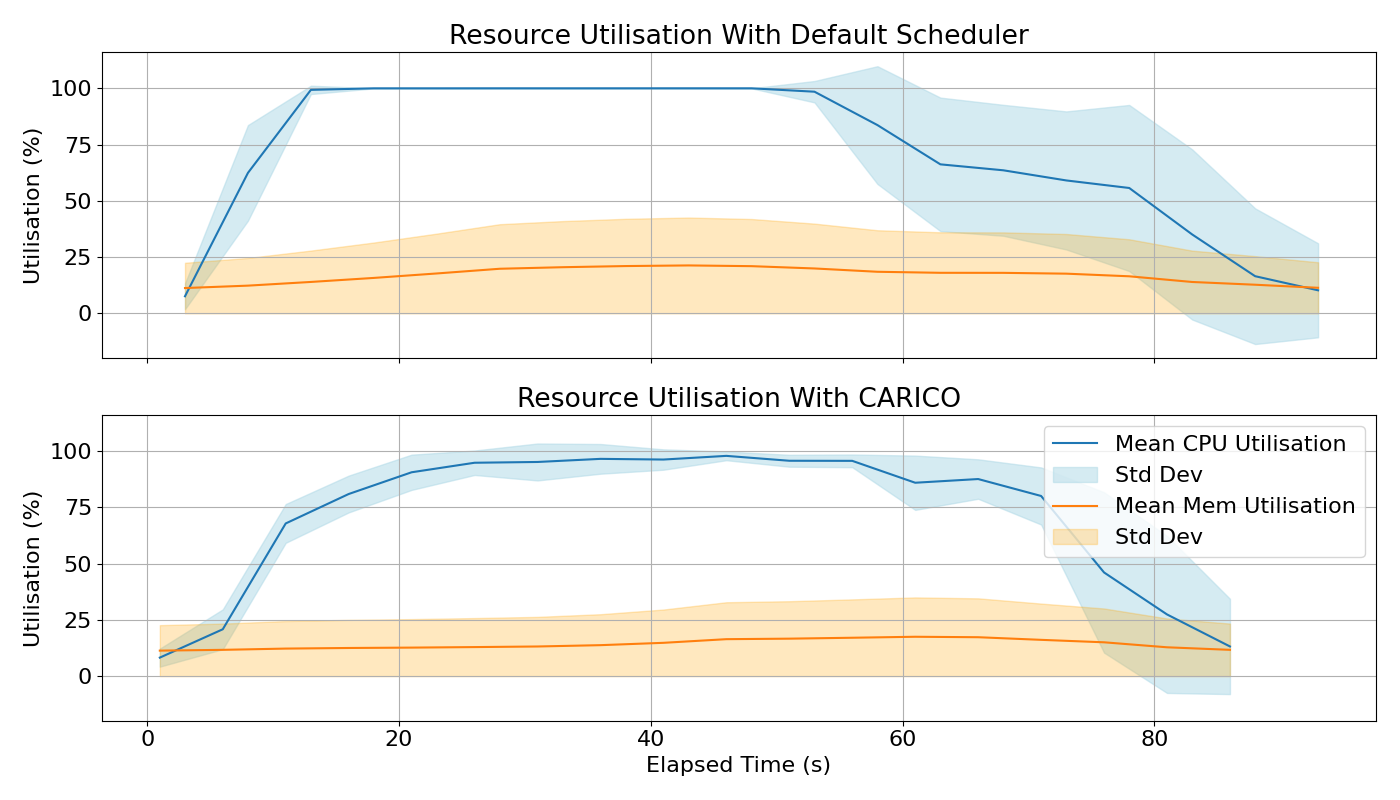
\includegraphics[width=\textwidth]{images/mixed-util.png}
    \caption{The resource utilisation when scheduling a Job with 1000 Pods
    executing \texttt{bpi(2000)}. The top figure gives the resource utilisation
    when scheduling with the default Kubernetes scheduler. The bottom figure
    gives the resource utilisation when scheduling with \textsc{Carico}.}
    \label{fig:mixed-util}
\end{figure}

Figure \ref{fig:mixed-util} shows the resource utilisation running the 500-20
combined Jobs. For the same reasons as with the  ML workload, the default
scheduler ends up with a low resource utilisation for the
latter portion of the Job exeuction. Instead, \textsc{Carico} achieves a more consistent
resource utilisations, experiencing less of a fall in CPU utilisation near the
end of the Job. In this scenario, \textsc{Carico} achieves a more efficient allocation of
resources.

\section{Workload Isolation}
\label{sec:workload-isolation}
To evaluate \textsc{Carico}'s QoS, I investigated how its scheduling decisions impact the
performance of already running Pods. For this experiment, I had a Pod running on
a worker Node, while another Pod periodically sent HTTP GET requests. This
polling Pod would then measure latency of the response. I then scheduled a Job
of 1000 Pods executing \texttt{bpi(2000)} across the cluster and measured how
the response latency changed. In the default schedulers case, each Pod requested
100 milliseconds of CPU time.

\begin{table}[h!]
\centering
    \begin{tabular}{|l|c|c|c|c|c|c|}
    \hline
    \textbf{Scenario} & \multicolumn{6}{c|}{\textbf{Response Latency (ms)}} \\
    \cline{2-7}
    & \textbf{Min} & \textbf{Med} & \textbf{P90} & \textbf{P95} & \textbf{P99} & \textbf{Max} \\
    \hline
    Baseline & 0.99 & 3.04 & 3.78 & 4.00 & 4.47 & 8.32 \\
    Default Scheduler & 1.07 & 10.06 & 18.61 & 22.28 & 28.82 & 54.49\\
    \textsc{Carico}  & 1.00 & 2.48 & 6.09 & 7.82 & 10.53 & 17.39\\
    \hline
    \end{tabular}
    \caption{The distribution of a servers response latency when different
    schedulers attempt to allocate a 1000 Pod Job across the server.}
    \label{tab:impacted-latency}
\end{table}

Table \ref{tab:impacted-latency} contains the measured distribution of the
response latency from the server. It shows how scheduling with the default
scheduler using 100m CPU requests, resulting a significant shift in latency
distribution. The median more than doubles and the distribution greatly shifted
towards the tail: the maximum latency was $\approx \times7$ larger. On the other
hand, when scheduling with \textsc{Carico}, the median latency actually decreased.
Furthermore, while the tail distribution did increase, the max latency was only
$\approx \times2$ bigger.

\section{Limitation}
\begin{tcolorbox}[boxsep=0mm,left=2.5mm,right=2.5mm]
    \textbf{Limitations:} {\em In this section, I will go over the limitations
    of the system. I will highlight how certain metrics like CPU-Utilisations
    don't give any more information once saturated. I will also have to mention
    how due to the sub-linear pod completion time, the Kubernetes scheduler is
    able to achieve higher job throughput by packing more pods into nodes.
    }
\end{tcolorbox}
% You've identified good points to include. The trade-off between CARICO's QoS benefits and potentially slightly lower raw throughput in some specific (e.g., CPU-bound, perfectly requested) scenarios for kube-scheduler is a key discussion point.
% Also consider limitations related to:
% The current set of metrics (CPU, Memory) and how CARICO might behave with I/O or network-bound workloads.
% The robustness of Kalman filter estimations to highly diverse pod types arriving in quick succession.
% Scalability of the flat aggregation server (though likely fine for your 20-node setup).

\section{Summary}
\begin{tcolorbox}[boxsep=0mm,left=2.5mm,right=2.5mm]
    \textbf{Summary:} {\em In this section, I will summarise the results of my
    evaluation section, highlighting key findings and reasoning.
    }
\end{tcolorbox}

